\section{Results}
\label{sec:wins}

DG's latency advantage is clear in serial mode. AR-30B takes
roughly one second to produce a 126-token JSON record; DG completes the
same task in under 400\,ms. If both models serve a security operations
centre processing alerts one at a time, DG handles \crossoverLambda{}
alerts per second per GPU, while AR-30B handles about one. AR stops at
its natural end-of-sequence token (EOS), so latency plateaus regardless
of \texttt{max\_tokens}.

Table~\ref{tab:niche} shows the serial comparison, AR-30B measured,
DG from the staircase law of Eq.~\ref{eq:dg}. The pattern reveals two
things: first, AR latency is flat from 128 tokens onward because the
model hits EOS, so setting \texttt{max\_tokens} higher has no effect.
Second, DG latency stays flat for the first canvas and then steps up
per additional canvas. The advantage is therefore non-monotonic: it
climbs to $2.5\times$ once AR reaches its natural length, then narrows
to $1.3\times$ by $L{=}1024$ as DG accrues canvas costs while AR
remains at its plateau. The $0.7\times$ in the first row is not a
like-for-like comparison: at \texttt{max\_tokens}${=}32$, AR is
truncated mid-record while DG still emits a full canvas. Extending the
same accounting past the table, the ratio keeps falling: $1.1\times$ at
$L{=}1280$ and $0.8\times$ at $L{=}2048$, where AR's plateau undercuts
DG's accumulated canvas cost. DG's serial advantage therefore holds at
typical output lengths but not universally.

\begin{table}[h]
\centering
\caption{Serial latency at the MoE-matched pair (AR-30B vs DG,
batch-1, BGL). AR-30B column is measured ($n{=}300$) and plateaus
because the model stops at $\sim$126 tokens (EOS), so raising
\texttt{max\_tokens} has no effect. The DG column is
Eq.~\ref{eq:dg} evaluated at the canvas count each budget implies,
anchored on the measured base ($n{=}300$) and canvas step
($n{=}200$). Forcing DG to fill those canvases measures 501\,ms at
$L{=}512$ and 739\,ms at $L{=}1024$, within 1\% of the law. The two
columns therefore compare AR at its natural output against DG at a
full canvas budget, a conservative reading for DG, which emits four
times more tokens at the last row.}
\label{tab:niche}
\begin{tabular}{@{}lrrrr@{}}
\toprule
max\_tokens & AR-30B (ms) & AR actual out & DG (ms) & DG advantage \\
\midrule
32   & 265  & 32  & 379 & $0.7\times$ \\
128  & 907  & 121 & 379 & $2.4\times$ \\
256  & 945  & 126 & 379 & $2.5\times$ \\
512  & 945  & 126 & 498 & $1.9\times$ \\
1024 & 945  & 126 & 737 & $1.3\times$ \\
\bottomrule
\end{tabular}
\end{table}

\paragraph{DG wins above the serial crossover.}

The serial cost law gives crossover $L^{*} = \crossoverL$ tokens; DG is
faster at any output length above $L^{*}$ (integer-safe: $L \geq 48$).
AR-30B serial slope (\arSlope\,ms/token) is $23\times$ steeper than its
batch-throughput slope. In batch mode the slope falls to
0.32\,ms/token (40.3\,ms/event over its natural output length at batch
300), because batch mode amortises prefill and decode overhead across
concurrent requests. Serial mode incurs that overhead per request.
Quoting a batch-throughput slope as if it were a latency therefore
understates AR serial latency by a factor of twenty-three.

\paragraph{Quality and latency.}

The latency comparison above uses the AR-30B MoE; the quality
comparison (\S\ref{sec:threats}) uses the dense AR-3B, the only
configuration with a measured quality CI. The AR-30B's own 9-field F1
is 0.870, slightly above the dense AR-3B's \arThreeBFnine, so the
latency advantage is conditional on the AR-30B being
quality-equivalent within that margin. The DG p50 is stable: a
bootstrap 95\% CI over 3{,}200 events spans [379, 380]\,ms. The AR-30B
p50 is 924\,ms with a bootstrap 95\% CI of [918, 927]\,ms over three
seeds ($n{=}900$ events). A permutation test on the difference of
medians (100\,k permutations) gives $p < 10^{-5}$, so the latency gap
is statistically significant. The AR-30B seed-to-seed CV is 0.04\%.
Figure~\ref{fig:distributions} shows the full per-event distributions.

\begin{figure}[ht!]
\centering
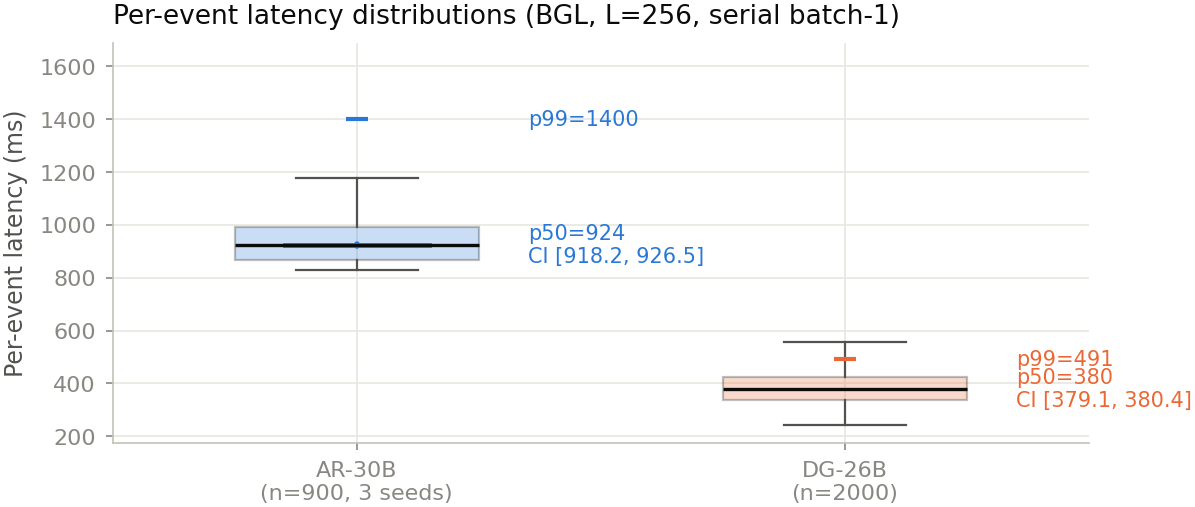
\includegraphics[width=0.85\linewidth]{figures/fig12_distributions.png}
\caption{Per-event latency distributions (BGL, $L{=}256$, serial
batch-1). Box plots show the full distribution; brackets mark the
bootstrap 95\% CI on the p50; crossbars mark p99. The AR-30B
distribution ($n{=}900$, three seeds pooled) is wider in absolute terms
but tighter in relative terms (max/median $1.75\times$ vs DG's
$3.07\times$). The non-overlapping CIs confirm the gap is significant
($p < 10^{-5}$, permutation test).}
\label{fig:distributions}
\end{figure}

\paragraph{Energy.}

DG uses less energy per event because it draws far less power above
idle: 10.8\,W net against the AR-30B's 173.3\,W. The cause is lower
power draw, not shorter busy time. In these two runs DG was in fact
busy longer per event. Denoising a canvas activates fewer compute units
than a token-by-token decode loop, so net power stays low even as
runtime grows. Over a million events the gap is 32\,kWh. The energy
ratio is:
\begin{equation}
R_{\mathrm{energy}} = \frac{E_{\mathrm{AR}}}{E_{\mathrm{DG}}}
\end{equation}
where $E_{\mathrm{AR}}$ and $E_{\mathrm{DG}}$ are the net energy per
event (joules, idle-subtracted) for each model. Measured values:
\begin{align}
\text{AR-30B MoE:} \quad & R_{\mathrm{energy}} =
\frac{118.7}{4.2} = 28.3 \quad \text{(idle 49.7\,W, serial)} \\
\text{Dense AR-1.5B:} \quad & R_{\mathrm{energy}} =
\frac{5.1}{4.2} = 1.2 \quad \text{(idle 58.6\,W)}
\end{align}
Both runs are now serial, matching the DG regime; the AR-30B's high
ratio reflects the 30B model's memory traffic during single-event
decode.

\paragraph{Graceful degradation under deadline pressure.}

Under a tightened deadline DG returns a complete canvas at lower
quality, while the AR model returns a truncated record that fails
schema validation. The $K$ knob is the difference: drop $K$ from 8 to 4
and the model still fills every field, just with slightly less
precision, instead of cutting the JSON in half mid-key. At a p99 budget
of 400\,ms, this meets it at \kFourPninetynine\,ms p99 with F1 falling
from \kEightFone\ to \kFourFone. Table~\ref{tab:contrast} summarises
the contrast across practical challenges.

\begin{table}[h]
\centering
\caption{Practical challenge contrast. Each row is a deployment
scenario; the right column names the architectural property that drives
the outcome. Every AR cell is the AR-30B MoE except the tail-latency
statistics, which use the dense AR-3B. The AR-30B's own tail
(max/med $1.75\times$, CV $12.3\%$) is tighter than DG's. Because that
model is dense, the tail asymmetry can't be attributed to MoE routing;
it's DG's denoising-step variance that drives it.}
\label{tab:contrast}
\begin{tabularx}{\linewidth}{@{}L L L L@{}}
\toprule
\thead{Challenge} & \thead{AR-30B MoE} & \thead{DG-26B MoE} & \thead{Key driver} \\
\midrule
Long output, batch-1 & \arSlope\,ms/token (serial) & Staircase, \dgStep\,ms/canvas & Crossover at $L^{*}\!\approx\!\crossoverL$ ($L\geq48$) \\
Deadline pressure & Truncates output & Drops $K$; complete canvas & Per-request quality parameter \\
High arrival rate & Batches $25\times$ & Caps at $\leq$1.7$\times$ & KV-cache reuse \\
Tail-sensitive service-level agreement (SLA) & Coefficient of variation (CV) \arEventCV\%, max/med \arMaxMed$\times$ (dense AR-3B) & CV \dgEventCV\%, max/med \dgMaxMed$\times$ & Denoising-step variance \\
Energy per event & 118.7\,J (serial) & 4.2\,J (serial) & Net power draw \\
Long prompt & Prefill paid once & Prefill paid $K$ times & Re-attention per step \\
\bottomrule
\end{tabularx}
\end{table}

The \dgMaxMed$\times$ tail violates a batch-1 SLA --- exactly the
regime where DG's per-event advantage applies (\S\ref{sec:limits}).
